%
% Copyright 2018 Joel Feldman, Andrew Rechnitzer and Elyse Yeager.
% This work is licensed under a Creative Commons Attribution-NonCommercial-ShareAlike 4.0 International License.
% https://creativecommons.org/licenses/by-nc-sa/4.0/
%

\questionheader{ex:s2.14}
%%%%%%%%%%%%%%%%%%
\subsection*{\Conceptual}
%%%%%%%%%%%%%%%%%%




\begin{question}What is the 180th derivative of the function $f(x)=e^x$?
\end{question}
\begin{hint} If you know the first derivative, this should be easy.
\end{hint}
\begin{answer} $e^x$
\end{answer}
\begin{solution} The derivative of $e^x$ is $e^x$: taking derivatives leaves the function unchanged, even if we do it 180 times. So $f^{(180)}=e^x$.
\end{solution}




\begin{Mquestion}
Suppose $f(x)$ is a differentiable function, with $f'(x)>0$ and $f''(x)>0$ for every $x \in (a,b)$. Which of the following must be true?
\begin{enumerate}[(i)]
\item\label{s2.14''i} $f(x)$ is positive over $(a,b)$
\item\label{s2.14''ii} $f(x)$ is increasing over $(a,b)$
\item\label{s2.14''iii} $f(x)$ is increasing at a constant rate over $(a,b)$
\item\label{s2.14''iv} $f(x)$ is increasing faster and faster over $(a,b)$
\item\label{s2.14''v} $f'''(x)>0$ for some $x \in (a,b)$
\end{enumerate}
\end{Mquestion}
\begin{hint} Exactly two of the statements must be true.
\end{hint}
\begin{answer}
\eqref{s2.14''ii}, \eqref{s2.14''iv}
\end{answer}
\begin{solution}
Since $f'(x)>0$ over $(a,b)$, we know from Corollary~\ref*{cor:DIFFmvtcons}
that $f(x)$ is increasing over $(a,b)$, so \eqref{s2.14''ii} holds. Since $f''(x)>0$, and $f''(x)$ is the derivative of $f'(x)$, by the same reasoning we see that $f'(x)$ is increasing. Since $f'(x)$ is the rate at which $f(x)$ is increasing, that means that the rate at which $f'(x)$ is increasing is itself increasing: this is, \eqref{s2.14''iv} holds (and \emph{not} \eqref{s2.14''iii}).

There is no reason to think \eqref{s2.14''i} or \eqref{s2.14''v} holds, but to be thorough we will give an example showing that they do not need to be true. If $f(x)=x^2-10$ and $(a,b)=(0,1)$, then $f'(x)=2x>0$ over $(0,1)$, and $f''(x)=2>0$ everywhere, but $f(x)<0$ for all $x \in (0,1)$, so \eqref{s2.14''i} does not hold. Also, $f'''(x)=0$ everywhere, so \eqref{s2.14''v} does not hold either.
\end{solution}







\begin{question}
Let $f(x)=ax^{15}$ for some constant $a$. Which value of $a$ results in $f^{(15)}(x)=3$?
\end{question}
\begin{hint}
Use factorials, as in Example~\ref*{eg:higherOrdDerivA}.
\end{hint}
\begin{answer}
$\dfrac{3}{15!}$
\end{answer}
\begin{solution}
Every time we differentiate $f(x)$, the constant out front gets multiplied by an ever-decreasing constant, while the power decreases by one. As in Example~\ref*{eg:higherOrdDerivA}, $\ds\ddiff{{15}}{}{x}ax^{15}=a\cdot 15!$. So, if $a\cdot 15!=3$, then $a=\dfrac{3}{15!}$.
\end{solution}




\begin{Mquestion}
Find the mistake(s) in the following work, and provide a corrected answer.
\begin{quote}
Suppose $-14x^2+2xy+y^2=1$. We find $\ds\ddiff{2}{y}{x}$ at the point $\left(1,3\right)$. Differentiating implicitly:
\begin{align*}
-28x+2y+2xy'+2yy'&=0
\intertext{Plugging in $x=1$, $y=3$:}
-28+6+2y'+6y'&=0\\
y'&=\frac{11}{4}
\intertext{Differentiating:}
y''&=0
\end{align*}
\end{quote}
\end{Mquestion}
\begin{hint}
The problem isn't with any of the algebra.
\end{hint}
\begin{answer}
The derivative $\ds\diff{y}{x}$ is $\dfrac{11}{4}$ only at the point $(1,3)$: it is not \emph{constantly} $\dfrac{11}{4}$, so it is wrong to differentiate the constant $\dfrac{11}{4}$ to find $\ds\ddiff{2}{y}{x}$. Below is a correct solution.
\begin{align*}
-28x+2y+2xy'+2yy'&=0
\intertext{Plugging in $x=1$, $y=3$:}
-28+6+2y'+6y'&=0\\
y'&=\frac{11}{4} \quad\mbox{\textcolor{red}{ at the point $(1,3)$}}
\intertext{Differentiating \textcolor{red}{the equation $-28x+2y+2xy'+2yy'=0$}:}
-28+2y'+2y'+2xy''+2y'y'+2yy''&=0\\
4y'+2(y')^2+2xy''+2yy''&=28
\intertext{At the point $(1,3)$, $y'=\dfrac{11}{4}$. Plugging in:}
4\left(\frac{11}{4}\right)+2\left(\frac{11}{4}\right)^2+2(1)y''+2(3)y''&=28\\
y''&=\frac{15}{64}
\end{align*}
\end{answer}
\begin{solution}
The derivative $\ds\diff{y}{x}$ is $\dfrac{11}{4}$ only at the point $(1,3)$: it is not \emph{constantly} $\dfrac{11}{4}$, so it is wrong to differentiate the constant $\dfrac{11}{4}$ to find $\ds\ddiff{2}{y}{x}$. Below is a correct solution.
\begin{align*}
-28x+2y+2xy'+2yy'&=0
\intertext{Plugging in $x=1$, $y=3$:}
-28+6+2y'+6y'&=0\\
y'&=\frac{11}{4} \quad\mbox{\textcolor{red}{ at the point $(1,3)$}}
\intertext{Differentiating \textcolor{red}{the equation $-28x+2y+2xy'+2yy'=0$}:}
-28+2y'+2y'+2xy''+2y'y'+2yy''&=0\\
4y'+2(y')^2+2xy''+2yy''&=28
\intertext{At the point $(1,3)$, $y'=\dfrac{11}{4}$. Plugging in:}
4\left(\frac{11}{4}\right)+2\left(\frac{11}{4}\right)^2+2(1)y''+2(3)y''&=28\\
y''&=\frac{15}{64}
\end{align*}
\end{solution}



%%%%%%%%%%%%%%%%%%
\subsection*{\Procedural}
%%%%%%%%%%%%%%%%%%



\begin{question}
Let $f(x)=(\log x-1)x$. Evaluate $f''(x)$.
\end{question}
\begin{hint}
Recall $\ds\diff{}{x}\log x =\ds\frac{1}{x}$.
\end{hint}
\begin{answer}
$f''(x)=\dfrac{1}{x}$
\end{answer}
\begin{solution}
\begin{align*}
f(x)&=x\log x -x\\
f'(x)&=\log x +x\cdot\frac{1}{x}-1\\
&=\log x\\
f''(x)&=\frac{1}{x}
\end{align*}
\end{solution}






\begin{Mquestion}
Evaluate $\ds\ddiff{2}{}{x}\{\arctan x\}$.
\end{Mquestion}
\begin{hint}
Recall $\ds\diff{}{x}\{\arctan x\}=\dfrac{1}{1+x^2}=(1+x^2)^{-1}$.
\end{hint}
\begin{answer}
$\ds\ddiff{2}{}{x}\{\arctan x\}=\frac{-2x}{(1+x^2)^2}$
\end{answer}
\begin{solution}
\begin{align*}
\diff{}{x}\{\arctan x\}&=\frac{1}{1+x^2}\\
\diff{}{x}\left\{\frac{1}{1+x^2}\right\}&=\diff{}{x}\left\{(1+x^2)^{-1}\right\}\\
&=(-1)(1+x^2)^{-2}(2x)\\&=\frac{-2x}{(1+x^2)^2}
\end{align*}
\end{solution}


\begin{question}
The unit circle consists of all point $x^2+y^2=1$. Give an expression for $\ds\ddiff{2}{y}{x}$ in terms of $y$.
\end{question}
\begin{hint}
Use implicit differentiation.
\end{hint}
\begin{answer}
$\ds\ddiff{2}{y}{x}=\dfrac{-1}{y^3}$
\end{answer}
\begin{solution}
We use implicit differentiation, twice.
\begin{align*}
2x+2yy'&=0\\
2+(2y)y''+(2y')y'&=0\\
y''&=-\frac{(y')^2+1}{y}
\intertext{So, we need an expression for $y'$. We use the equation $2x+2yy'=0$ to conclude $y'=-\dfrac{x}{y}$:}
y''&=-\frac{\left(-\frac{x}{y}\right)^2+1}{y}\\
&=-\frac{\frac{x^2}{y^2}+1}{y}\\
&=-\frac{x^2+y^2}{y^3}\\
&=-\frac{1}{y^3}
\end{align*}
\end{solution}


\begin{Mquestion}
Suppose the position of a particle at time $t$ is given by $s(t) = \dfrac{e^t}{t^2+1}$. Find the acceleration of the particle at time $t=1$.
\end{Mquestion}
\begin{hint}
The acceleration is given by $s''(t)$.
\end{hint}
\begin{answer}
$0$
\end{answer}
\begin{solution}
The question asks for $s''(1)$. We start our differentiation using the quotient rule:
\begin{align*}
s'(t)&=\frac{e^t(t^2+1)-e^t(2t)}{(t^2+1)^2}\\
&=\frac{e^t(t^2-2t+1)}{(t^2+1)^2}
\intertext{Using the quotient rule again,}
s''(t)&=\frac{(t^2+1)^2\textcolor{blue}{\diff{}{t}\{e^t(t^2-2t+1)\}}-e^t(t^2-2t+1) \textcolor{red}{\diff{}{t}\{(t^2+1)^2\}}}{(t^2+1)^4}\\
&=\frac{(t^2+1)^2\cdot\left[\textcolor{blue}{e^t(2t-2)+e^t(t^2-2t+1)}\right]-
e^t(t^2-2t+1) \cdot \textcolor{red}{2(t^2+1)(2t)}}{(t^2+1)^4}\\
&=\frac{e^t(t^2+1)^2(t^2-1)-4te^t(t-1)^2(t^2+1)}{(t^2+1)^4}\\
s''(1)&=0
\end{align*}
\end{solution}



\begin{question}
Evaluate $\ds\ddiff{3}{}{x}\{\log(5x^2-12)\}$.
\end{question}
\begin{hint}
Remember to use the chain rule.
\end{hint}
\begin{answer}
$\ds\ddiff{3}{}{x}\{\log(5x^2-12)\}=\frac{100x(5x^2+36)}{(5x^2-12)^3}$
\end{answer}
\begin{solution}
We differentiate using the chain rule.
\begin{align*}
\diff{}{x}\{\log(5x^2-12)\}&=\frac{10x}{5x^2-12}
\intertext{Using the quotient rule:}
\ddiff{2}{}{x}\{\log(5x^2-12)\}&=\diff{}{x}\left\{\frac{10x}{5x^2-12}\right\}\\
&=\frac{(5x^2-12)(10)-10x(10x)}{(5x^2-12)^2}\\
&=\frac{-10(5x^2+12)}{(5x^2-12)^2}
\intertext{Using the quotient rule one last time:}
\ddiff{3}{}{x}\{\log(5x^2-12)\}&=\diff{}{x}\left\{
\frac{-10(5x^2+12)}{(5x^2-12)^2}
\right\}\\
&=\frac{(5x^2-12)^2(-10)(10x)+10(5x^2+12)(2)(5x^2-12)(10x)}{(5x^2-12)^4}\\
&=\frac{(5x^2-12)(-100x)+(200x)(5x^2+12)}{(5x^2-12)^3}\\
&=\frac{100x(-5x^2+12+10x^2+24)}{(5x^2-12)^3}\\
&=\frac{100x(5x^2+36)}{(5x^2-12)^3}
\end{align*}
\end{solution}






\begin{question}
The height of a particle at time $t$ seconds is given by $h(t)=-\cos t$. Is the particle speeding up or slowing down at $t=1$?
\end{question}
\begin{hint}
$h'(t)$ gives the velocity of the particle, and $h''(t)$ gives its acceleration--the rate the velocity is changing.
\end{hint}
\begin{answer}
speeding up
\end{answer}
\begin{solution}
The velocity of the particle is given by $h'(t)=\sin t$. Note $0<1<\pi$, so
$h'(1)>0$--the particle is rising (moving in the positive direction, in this case ``up").
The acceleration of the particle is $h''(t)=\cos t$. Since $0<1<\frac{\pi}{2}$, $h''(t)>0$, so $h'(t)$ is increasing: the particle is moving up, and it's doing so at an increasing rate. So, the particle is speeding up.
\end{solution}

\begin{Mquestion}
The height of a particle at time $t$ seconds is given by $h(t)=t^3-t^2-5t+10$. Is the particle's motion getting faster or slower at $t=1$?
\end{Mquestion}
\begin{hint}
$h'(t)$ gives the velocity of the particle, and $h''(t)$ gives its acceleration--the rate the velocity is changing. Be wary of signs--as in legends, they may be misleading.
\end{hint}
\begin{answer}
slower
\end{answer}
\begin{solution}
For this problem, remember that velocity has a sign indicating direction, while speed does not.

The velocity of the particle is given by $h'(t)=3t^2-2t-5$. At $t=1$, the velocity of the particle is $-4$, so the particle is moving downwards with a speed of 4 units per second. The acceleration of the particle is $h''(t)=6t-2$, so when $t=1$, the acceleration is (positive) $4$ units per second per second. That means the velocity (currently $-4$ units per second) is becoming a bigger number--since the velocity is negative, a bigger number is closer to zero, so the speed of the particle is getting smaller. (For instance, a velocity of $-3$ represents a slower motion than a velocity of $-4$.) So, the particle is  slowing down at $t=1$.
\end{solution}



\begin{question}
Suppose a curve is defined implicitly by
\[x^2+x+y=\sin(xy)\]
What is $\ds\ddiff{2}{y}{x}$ at the point $(0,0)$?
\end{question}
\begin{hint}
You don't need to solve for $y''$ in general--only when $x=y=0$. To do this, you \emph{also} need to find $y'$ at the point $(0,0)$.
\end{hint}
\begin{answer}
$-4$
\end{answer}
\begin{solution}
\begin{align*}
x^2+x+y&=\sin(xy)
\intertext{We differentiate implicitly. For ease of notation, we write $y'$ for $\ds\diff{y}{x}$.}
2x+1+y'&=\cos(xy)(y+xy')
\intertext{We're interested in $y''$, so we implicitly differentiate again.}
2+y''&=-\sin(xy)(y+xy')^2+\cos(xy)(2y'+xy'')
\intertext{We want to know what $y''$ is when $x=y=0$. Plugging these in yields the following:}
2+y''&=2y'
\intertext{So, we need to know what $y'$ is when $x=y=0$. We can get this from the equation $2x+1+y'=\cos(xy)(y+xy')$, which becomes
$1+y'=0$ when $x=y=0$. So, at the origin, $y'=-1$, and}
2+y''&=2(-1)\\
y''&=-4
\end{align*}
Remark: a common mistake is to stop at the equation
$2x+1+y'=\cos(xy)(y+xy')$, plug in $x=y=0$, find $y'=-1$, and decide $y''=\ds\diff{}{x}\{-1\}=0$. This is due to a slight sloppiness in the usual notation. When we wrote $y'=1$, what we meant is that \emph{at the point} $(0,0)$, $\ds\diff{y}{x}=-1$. More properly written: $\left.\ds\diff{y}{x}\right|_{x=0,~y=0}=-1$. This is not the same as saying $y'=1$ everywhere (in which case, indeed, $y''$ would be 0 everywhere).
\end{solution}





\begin{Mquestion}
Which statements below are true, and which false?
\begin{enumerate}[(a)]
\item $\ds\ddiff{4}{}{x} \sin x = \sin x$
\item $\ds\ddiff{4}{}{x} \cos x = \cos x$
\item $\ds\ddiff{4}{}{x} \tan x = \tan x$
\end{enumerate}
\end{Mquestion}
\begin{hint}
To show that two functions are unequal, you can show that one input results in different outputs.
\end{hint}
\begin{answer}
(a) true \qquad (b) true \qquad (c) false
\end{answer}
\begin{solution}
For (a) and (b), notice the following:
\begin{align*}
\diff{}{x} \sin x &= \cos x\\
\diff{}{x} \cos x &= -\sin x\\
\diff{}{x} \{-\sin x\} &= -\cos x\\
\diff{}{x} \{-\cos x\} &= \sin x\\
\diff{}{x} \sin x &= \cos x
\intertext{The fourth derivative is $\sin x$ is $\sin x$, and the fourth derivative of $\cos x$ is $\cos x$, so (a) and (b) are true.}
\diff{}{x}\tan x &=\sec^2 x\\
\diff{}{x}\sec^2 x &=2\sec x (\sec x \tan x)=2\sec^2x\tan x\\
\diff{}{x}\{2\sec^2x\tan x\}&=(4\sec x \cdot \sec x \tan x)\tan x+2\sec^2x\sec^2x\\
&=4\sec^2x\tan^2x+2\sec^4x\\
\diff{}{x}\{4\sec^2x\tan^2x+2\sec^4x\}&=(8\sec x \cdot \sec x \tan x)\tan^2x+4\sec^2x(2\tan x \cdot\sec^2x)\\&\quad+8\sec^3x\cdot\sec x \tan x\\
&=8\sec^2x\tan^3x+16\sec^4x\tan x
\end{align*}
So, $\ds\ddiff{4}{}{x} \tan x =8\sec^2x\tan^3x+16\sec^4x\tan x$. It certainly seems like this is not the same as $\tan x$, but remember that sometimes trig identities can fool you: $\tan^2x+1=\sec^2x$, and so on. So, to be absolutely sure that these are not equal, we need to find a value of $x$ so that the output of one is not the same as the output of the other. When $x=\frac{\pi}{4}$:
\[8\sec^2x\tan^3x+16\sec^4x\tan x = 8\left({\sqrt{2}}\right)^2(1)^3+16\left({\sqrt{2}}\right)^4(1)=80\neq 1=\tan x.\]
So, (c) is false.
\end{solution}




%%%%%%%%%%%%%%%%%%
\subsection*{\Application}
%%%%%%%%%%%%%%%%%%

\begin{Mquestion}
A function $f(x)$ satisfies $f'(x)<0$ and $f''(x)>0$ over $(a,b)$. Which of the following curves below might represent $y=f(x)$?
\begin{center}
\begin{tikzpicture}
\YEaaxis{1}{3}{1}{2}
\YExcoord{.5}{a}
\YExcoord{2.5}{b}
\draw[thick] plot[domain=.5:2.5](\x,{\x*\x*\x*\x/35+.5});
\draw (1.5,-1.5) node{(i)};
\end{tikzpicture}\hfill
\begin{tikzpicture}
\YEaaxis{1}{3}{1}{2}
\YExcoord{.5}{a}
\YExcoord{2.5}{b}
\draw[thick] plot[domain=.5:2.5](3-\x,{\x*\x*\x*\x/35+.5});
\draw (1.5,-1.5) node{(ii)};
\end{tikzpicture}\hfill
\begin{tikzpicture}
\YEaaxis{1}{3}{1}{2}
\YExcoord{.5}{a}
\YExcoord{2.5}{b}
\draw[thick] plot[domain=.5:2.5](\x,{1.5-\x*\x*\x*\x/35});
\draw (1.5,-1.5) node{(iii)};
\end{tikzpicture}

\hfill
\begin{tikzpicture}
\YEaaxis{1}{3}{1}{2}
\YExcoord{.5}{a}
\YExcoord{2.5}{b}
\draw[thick] plot[domain=.5:2.5](3-\x,{1.5-\x*\x*\x*\x/35+.5});
\draw (1.5,-1.5) node{(iv)};
\end{tikzpicture}\hfill
\begin{tikzpicture}
\YEaaxis{1}{3}{1}{2}
\YExcoord{.5}{a}
\YExcoord{2.5}{b}
\draw[thick] plot[domain=.5:2.5](\x,{2.25-\x*.75});
\draw (1.5,-1.5) node{(v)};
\end{tikzpicture}
\hfill~
\end{center}
\end{Mquestion}
\begin{hint} Only one of the curves could possibly represent $y=f(x)$.
\end{hint}
\begin{answer} (ii)
\end{answer}
\begin{solution}
Since $f'(x)<0$, we need a decreasing function. This only applies to (ii), (iii), and  (v). Since $f''(x)>0$, that means $f'(x)$ is increasing, so the \emph{slope} of the function must be increasing. In (v), the slope is constant, so $f''(x)=0$--therefore, it's not (v).
In (iii), the slope is decreasing, because near $a$ the curve is quite flat ($f'(x)$ near zero) but near $b$ the curve is very steeply decreasing ($f'(x)$ is a large \emph{negative} number), so (iii) has a negative second derivative. By contrast, in (ii), the line starts out as steeply decreasing ($f'(x)$ is a strongly negative number) and becomes flatter and flatter ($f'(x)$ nears 0), so $f'(x)$ is increasing--in other words, $f''(x)>0$. So, (ii) is the only curve that has $f'(x)<0$ and $f''(x)>0$.
\end{solution}



\begin{question}
Let $f(x)=2^{x}$. What is $f^{(n)}(x)$, if $n$ is a whole number?
\end{question}
\begin{hint}
Remember $\ds\diff{}{x}\{2^x\}=2^x\log2$.
\end{hint}
\begin{answer}
$f^{(n)}=2^x(\log 2)^n$
\end{answer}
\begin{solution}
We differentiate a few time to find the pattern.
\begin{align*}
\diff{}{x}\{2^x\}&=2^x\log 2\\
\ddiff{2}{}{x}\{2^x\}&=2^x\log2 \cdot \log 2 = 2^x(\log2)^2\\
\ddiff{3}{}{x}\{2^x\}&=2^x(\log2)^2 \cdot \log 2 = 2^x(\log2)^3
\intertext{Every time we differentiate, we multiply the original function by another factor of $\log 2$. So, the $n$th derivative is given by:}
\ddiff{n}{}{x}\{2^x\}&=2^x(\log2)^n
\end{align*}
\end{solution}



\begin{Mquestion}
Let $f(x)=ax^3+bx^2+cx+d$, where $a$, $b$, $c$, and $d$ are nonzero constants.
What is the smallest integer $n$ so that $\ds\ddiff{n}{f}{x}=0$ for all $x$?
\end{Mquestion}
\begin{hint}
Differentiate a few times until you get zero, remembering that $a$, $b$, $c$, and $d$ are all constants.
\end{hint}
\begin{answer}
 $n=4$
\end{answer}
\begin{solution}
We differentiate using the power rule.
\begin{align*}
\diff{f}{x}&=3ax^2+2bx+c\\
\ddiff{2}{f}{x}&=6ax+2b\\
\ddiff{3}{f}{x}&=6a\\
\ddiff{4}{f}{x}&=0
\end{align*}
In the above work, remember that $a$, $b$, $c$, and $d$ are all constants. Since they are nonzero constants, $\ds\ddiff{3}{f}{x} =6a\neq 0$. So, the fourth derivative is the first derivative to be identically zero: $n=4$.
\end{solution}


\begin{question}[1999H]
\[f(x)=e^{x+x^2}\qquad \qquad \qquad h(x)=1+x+\frac{3}{2}x^2\]
\begin{enumerate}[(a)]
\item\label{s2.14ineq1} Find the first and second derivatives of both functions
\item\label{s2.14ineq2} Evaluate both functions and their first and second derivatives at 0.
\item\label{s2.14ineq3} Show that for all $x>0$, $f(x)>h(x)$.
\end{enumerate}
Remark: for some applications, we only need to know that a function is ``big enough." Since $f(x)$ is a difficult function to evaluate, it may be useful to know that it is bigger than $h(x)$ when $x$ is positive.
\end{question}
\begin{hint} Use a similar method to Question~\ref{s2.9ineq}, Section~\ref*{sec chain rule}.
\end{hint}
\begin{answer}
\eqref{s2.14ineq1} $f'(x)=(1+2x)e^{x+x^2}$ \quad $f''(x)=(4x^2+4x+3)e^{x+x^2}$\quad
 $h'(x)=1+3x$ \quad $h''(x)=3$\\
\eqref{s2.14ineq2} $f(0)=h(0)=1$; \quad $f'(0)=h'(0)=1$; \quad $f''(0)=h''(0)=3$\\
\eqref{s2.14ineq3} $f$ and $h$ ``start at the same place," since $f(0)=h(0)$. Also $f'(0)=h'(0)$, and $f''(x)=(4x^2+4x+3)e^{x+x^2} > 3e^{x+x^2}>3=h''(x)$ when $x>0$. Since $f'(0)=h'(0)$, and since $f'$ grows faster than $h'$ for positive $x$, we conclude $f'(x)>h'(x)$ for all positive $x$. Now we can conclude that (since $f(0)=h(0)$ and $f$ grows faster than $h$ when $x>0$) also $f(x)>h(x)$ for all positive $x$.
\end{answer}
\begin{solution}
\eqref{s2.14ineq1}
Using the chain rule for $f(x)$:
\begin{align*}
f'(x)&=(1+2x)e^{x+x^2}\\
f''(x)&=(1+2x)(1+2x)e^{x+x^2}+(2)e^{x+x^2}=(4x^2+4x+3)e^{x+x^2}\\
h'(x)&=1+3x\\
h''(x)&=3
\end{align*}

\eqref{s2.14ineq2} $f(0)=h(0)=1$; \quad $f'(0)=h'(0)=1$; \quad $f''(0)=h''(0)=3$\\
\eqref{s2.14ineq3} $f$ and $h$ ``start at the same place," since $f(0)=h(0)$. If it were clear that $f'(x)$ were greater than $h'(x)$ for $x>0$, then we  would know that $f$ grows faster than $h$, so we could conclude that $f(x)>h(x)$, as desired. Unfortunately, it is not obvious whether $(1+2x)e^{x+x^2}$ is always greater than $1+3x$ for positive $x$. So, we look to the second derivative. $f'(0)=h'(0)$, and $f''(x)=(4x^2+4x+3)e^{x+x^2} > 3e^{x+x^2}>3=h''(x)$ when $x>0$. Since $f'(0)=h'(0)$, and since $f'$ grows faster than $h'$ for positive $x$, we conclude $f'(x)>h'(x)$ for all positive $x$. Now we can conclude that (since $f(0)=h(0)$ and $f$ grows faster than $h$ when $x>0$) also $f(x)>h(x)$ for all positive $x$.
\end{solution}


\begin{question}[1997D]
 The equation $x^3y+y^3=10x$ defines $y$ implicitly as a function
of $x$ near the point $(1,2)$.
\begin{enumerate}[(a)]
\item\label{s2.11p2.1} Compute $y'$ at this point.
\item\label{s2.11p2.2} It can be shown that $y''$ is negative when $x=1$. Use this
fact and your answer to \eqref{s2.11p2.1} to make a sketch showing the relationship of
the curve to its tangent line at $(1,2)$.
\end{enumerate}
\end{question}
\begin{hint} For \eqref{s2.11p2.2}, you know a point where the curve and tangent line intersect, and you know what the tangent line looks like. What do the derivatives tell you about the shape of the curve?
\end{hint}
\begin{answer}
\begin{enumerate}[(a)]
\item $y'(1)=\dfrac{4}{13}$
\item ~
\begin{center}
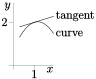
\includegraphics{graphE3}
\end{center}
\end{enumerate}
\end{answer}
\begin{solution}
\begin{enumerate}[(a)]
\item
We differentiate implicitly.
\begin{align*}
x^3y(x)+y(x)^3&=10 x\\
3x^2y(x)+x^3y'(x)+3y(x)^2y'(x)&=10
\intertext{Subbing in $x=1$ and $y(1)=2$ gives}
(3)(1)( 2)+(1)y'(1)+(3)(4) y'(1)&=10\\
13y'(1)&=4\\
y'(1)&=\frac{4}{13}
\end{align*}

\item
 From part \eqref{s2.11p2.1}, the slope of the curve at $x=1,\ y=2$ is $\dfrac{4}{13}$,
so the curve is increasing, but fairly slowly. The angle of the tangent
line is $\tan^{-1}\left(\frac{4}{13}\right)\approx 17^\circ$. We are also told that $y''(1)<0$.
So the slope of the curve is decreasing as $x$ passes through 1. That is, the line is more steeply increasing to the left of $x=1$, and its slope is decreasing (getting less sleep, then possibly the slope even becomes negative) as we move past $x=1$.
%\figput{graphE3}
\begin{center}
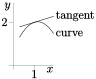
\includegraphics{graphE3}
\end{center}
\end{enumerate}
\end{solution}


\begin{question}\label{s2.14expprod}
Let $g(x)=f(x)e^x$.
In Question~\ref{s2.7expprod}, Section~\ref*{sec exp func}, we learned that $g'(x)=[f(x)+f'(x)]e^x$.
\begin{enumerate}[(a)]
\item\label{s2.14expprod1} What is $g''(x)$?
\item\label{s2.14expprod2} What is $g'''(x)$?
\item\label{s2.14expprod3} Based on your answers above, guess a formula for $g^{(4)}(x)$. Check it by differentiating.
\end{enumerate}
\end{question}
\begin{hint}
Review Pascal's Triangle.
\end{hint}
\begin{answer}
\eqref{s2.14expprod1} $g''(x)=[f(x)+2f'(x)+f''(x)]e^x$\\
\eqref{s2.14expprod2}  $g'''(x)=[f(x)+3f'(x)+3f''(x)+f'''(x)]e^x$\\
\eqref{s2.14expprod3} $g^{(4)}(x)=[f(x)+4f'(x)+6f''(x)+4f'''(x)+f^{(4)}(x)]e^x$
\end{answer}
\begin{solution}
\eqref{s2.14expprod1} Using the product rule, \[g''(x)=[f'(x)+f''(x)]e^x+[f(x)+f'(x)]e^x=[f(x)+2f'(x)+f''(x)]e^x\]

\eqref{s2.14expprod2}  Using the product rule and our answer from~\eqref{s2.14expprod1},
\begin{align*}
g'''(x)&=[f'(x)+2f''(x)+f'''(x)]e^x+[f(x)+2f'(x)+f''(x)]e^x\\
&=[f(x)+3f'(x)+3f''(x)+f'''(x)]e^x
\end{align*}

\eqref{s2.14expprod3} We notice that the coefficients of the derivatives of $f$ correspond to the entries in the rows of Pascal's Triangle.
\begin{center}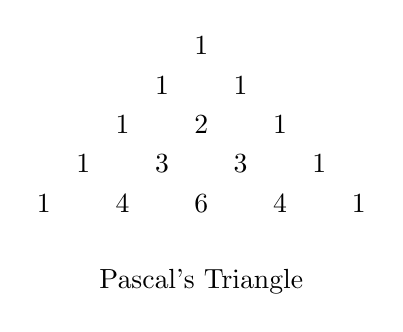
\begin{tikzpicture}
\draw (0,3) node{1};
\draw (-.5,2.5) node{1}; \draw (.5,2.5) node{1};
\draw (-1,2) node{1}; \draw (1,2) node{1}; \draw (0,2) node{2};
\draw (-1.5,1.5) node{1}; \draw (1.5,1.5) node{1}; \draw (-.5,1.5) node{3}; \draw (.5,1.5) node{3};
\draw (-2,1) node{1}; \draw (2,1) node{1}; \draw (-1,1) node{4}; \draw (1,1) node{4}; \draw (0,1) node{6};
\draw (0,0) node{Pascal's Triangle};
\end{tikzpicture}\end{center}
\begin{itemize}
\item In the first derivative of $g$, the coefficients of $f$ and $f'$ correspond to the entries in the second row of Pascal's Triangle.
\item In the second derivative of $g$, the coefficients of $f$, $f'$, and $f''$ correspond to the entries in the third row of Pascal's Triangle.
\item In the third derivative of $g$, the coefficients of $f$, $f'$, $f''$, and $f'''$ correspond to the entries in the fourth row of Pascal's Triangle.
\item We guess that, in the fourth derivative of $g$, the coefficients of $f$, $f'$, $f''$, $f'''$, and $f^{(4)}$ will correspond to the entries in the fifth row of Pascal's Triangle.
\end{itemize}
That is, we guess
\[g^{(4)}(x)=[f(x)+4f'(x)+6f''(x)+4f'''(x)+f^{(4)}(x)]e^x\]
This is verified by differentiating our answer from \eqref{s2.14expprod1} using the product rule:
\begin{align*}
g'''(x)&=[f(x)+3f'(x)+3f''(x)+f'''(x)]e^x\\
g^{(4)}(x)&=[f'(x)+3f''(x)+3f'''(x)+f^{(4)}(x)]e^x+[f(x)+3f'(x)+3f''(x)+f'''(x)]e^x\\
&=[f(x)+4f'(x)+6f''(x)+4f'''(x)+f^{(4)}(x)]e^x.
\end{align*}
\end{solution}

\begin{question}\label{s2.14rollemultipleroots}
Suppose $f(x)$ is a function whose first $n$ derivatives exist over all real numbers, and $f^{(n)}(x)$ has precisely $m$ roots. What is the maximum number of roots that $f(x)$ may have?
\end{question}
\begin{hint}
Rolle's Theorem relates the roots of a function to the roots of its derivative. So, the fifth derivative tells us something about the fourth, the fourth derivative tells us something about the third, and so on.
\end{hint}
\begin{answer}
$m+n$
\end{answer}
\begin{solution}
Since $f(x)$ is differentiable over all real numbers, it is also continuous over all real numbers. Similarly, $f'(x)$ is differentiable over all real numbers, so it is also continuous over all real numbers, and so on for the first $n$ derivatives of $f(x)$.

Rolle's Theorem tells us that if $a$ and $b$ are distinct roots of a function $g$, then $g'(x)=0$ for some $c$ in $(a,b)$. That is, $g'$ has a root strictly between $a$ and $b$. Expanding this idea, if $g$ has $m+1$ distinct roots, then $g'$ must have at least $m$ distinct roots, as in the sketch below.

\begin{center}
\begin{tikzpicture}
\draw[ultra thick, <->] (0,0)--(10,0);
\color{blue}
\draw (1,.2)--(1,-.2) node[below](a1){$a_1$};
\draw (3,.2)--(3,-.2) node[below](a2){$a_2$};
\draw (5,.2)--(5,-.2) node[below](a3){$a_3$};
\draw (9,.2)--(9,-.2) node[below](a4){$a_{m+1}$};
\draw (3,-3) node(b){roots of $g(x)$};
\foreach \x in {1,2,3,4} {\draw[dashed, ->] (b)--(a\x);}
\color{red}
\draw (2,-.2)--(2,.2) node[above](c1){$c_1$};
\draw (4,-.2)--(4,.2) node[above](c2){$c_2$};
\draw (8,-.2)--(8,.2) node[above](c3){$c_{m}$};
\draw (3,3) node(c){roots of $g'(x)$};
\foreach \x in {1,2,3} {\draw[dashed, ->] (c)--(c\x);}
\end{tikzpicture}\end{center}

So, if $f^{(n)}(x)$ has only $m$ roots, then $f^{(n-1)}(x)$ has at most $m+1$ roots. Similarly, since $f^{(n-1)}(x)$ has at most $m+1$ roots, $f^{(n-2)}(x)$ has at most $m+2$ roots. Continuing in this way, we see $f(x)=f^{(n-n)}(x)$ has at most $m+n$ distinct roots.
\end{solution}



\begin{question}
How many roots does the function $f(x)=(x+1)\log(x+1)+\sin x - x^2$ have?
\end{question}
\begin{hint}
You'll want to use Rolle's Theorem, but the first derivative won't be very tractable--use  the idea behind Question~\ref{s2.14rollemultipleroots}.
\end{hint}
\begin{answer}
$2$
\end{answer}
\begin{solution}
\begin{itemize}
\item Let's begin by noticing that the domain of $f(x)$ is $(-1,\infty)$.
\item By inspection, $f(0)=0$, so $f(x)$ has at least one root.
\item If $x\in(-1,0)$, then $(x+1)$ is positive, $\log(x+1)$ is negative,  $\sin(x)$ is negative, and $-x^2$ is negative. Therefore, if $x<0$ is in the domain of $f$, then $f(x)<0$. So, $f(x)$ has no negative roots. We focus our attention on the case $x>0$.
\item $f'(x)=1-2x+\log(x+1)+\cos x$.  We would like to know how many positive roots $f'(x)$ has, but it isn't obvious. So, let's differentiate again.
\item $f''(x)=-2+\frac{1}{x+1}-\sin x$. When $x>0$, $\frac{1}{x+1}<1$, so $f''(x) <-1-\sin(x) \leq 0$, so $f''(x)$ has \emph{no positive roots}. Since $f'(x)$ is continuous and differentiable over $(0,\infty)$, and since $f''(x) \neq 0$ for all $x \in (0, \infty)$, by Rolle's Theorem, $f'(x)$ has at most one root in $[0,\infty)$.
\item Since $f(x)$ is continuous and differentiable
over $[0,\infty)$, and $f'(x)$ has at most one root in $(0,\infty)$, by Rolle's Theorem $f(x)$ has at most two distinct roots in $[0,\infty)$.
(Otherwise, $f(a)=f(b)=f(c)=0$ for some values $0\le a<b<c$, so $f'(d)=f'(e)=0$ for some $d\in(a,b)$ and some $e \in (b,c)$, but since $f'(x)$ has at most one root, this is impossible.)
\item We know $f(0)=0$, so the remaining question is whether or not $f(x)$ has a second root (which would have to be positive). As usual, we can show another root exists using the intermediate value theorem. We see that for large values of $x$, $f(x)$ is negative, for example:
\[f(4)=5\log 5+\sin(4)-(4)^2 <  5\log(e^2) + 1 -16 =11-16<0\]
For positive values of $x$ closer to zero, we hope to find a positive value of $f(x)$.
However, it's quite difficult to get a number $c$ that obviously gives $f(c)>0$.
It suffices to observe that $f(0)=0$ and $f'(0)=2>0$. From the definition of the derivative, we can conclude $f(x)>0$ for some $x>0$. (If it is not true that $f(x)>0$ for some $x>0$, then $f(x)\le 0$
      for all $x>0$. The definition of the derivative tells us that [since $f'(0)$ exists]
 $f'(0)=\ds\lim_{h \to 0^+}\frac{f(h)-f(0)}{h}=\ds\lim_{h \to 0^+}\frac{f(h)}{h}$; the denominator is positive, so if the numerator were always less than or equal to zero, the limit would be less than or equal to zero as well. However, the derivative is positive, so $f(x)>0$ for some $x>0$.)
Therefore, $f(x)$ has a second root, so $f(x)$ has precisely two roots.
\end{itemize}
\end{solution}







\begin{Mquestion}[2007H]
Let $f(x) = x|x|$.
\begin{enumerate}[(a)]
\item\label{s2.14_2007_1} Show that
$f(x)$ is differentiable at $x = 0$, and find $f'(0)$.
\item\label{s2.14_2007_2} Find the second derivative of $f(x)$. Explicitly state,
with justification, the point(s) at which $f''(x)$ does not exist, if any.
\end{enumerate}
\end{Mquestion}
\begin{hint} You can re-write this function as a piecewise function, with branches $x \ge 0$ and $x<0$. To figure out the derivatives at $x = 0$, use
          the definition of a derivative.
\end{hint}
\begin{answer}
\eqref{s2.14_2007_1}
In order to make $f(x)$ a little more tractable, let's change the format. Since
$|x|=\left\{\begin{array}{rl}
x&x \geq 0\\
-x&x<0
\end{array}\right.$, then:
\[f(x)=\left\{\begin{array}{rl}
-x^2&x<0\\
x^2&x\ge 0.\end{array}
\right. \]

Now, we turn to the definition of the derivative to figure out whether $f'(0)$ exists.
\begin{align*}
f'(0)&=\lim_{h \to 0} \frac{f(0+h)-f(0)}{h}=\lim_{h \to 0}\frac{f(h)-0}{h} =\lim_{h \to 0}\frac{f(h)}{h}\qquad\mbox{if it exists.}
\intertext{Since $f$ looks different to the left and right of 0, in order to evaluate this limit, we look at the corresponding one-sided limits. Note that when $h$ approaches 0 from the right, $h>0$ so $f(h)=h^2$.
By contrast, when $h$ approaches 0 from the left, $h<0$ so $f(h)=-h^2$.}
&~\lim_{h \to 0^+} \frac{f(h)}{h}=\lim_{h \to 0^+}\frac{h^2}{h}=\lim_{h \to 0^+}h=0\\
&~\lim_{h \to 0^-} \frac{f(h)}{h}=\lim_{h \to 0^-}\frac{-h^2}{h}=\lim_{h \to 0^-}-h=0
\intertext{Since both one-sided limits exist and are equal to 0,}
&~\lim_{h \to 0} \frac{f(0+h)-f(0)}{h}=0
\end{align*}
and so $f$ is differentiable at $x=0$ and $f'(0)=0$.

\eqref{s2.14_2007_2}
From \eqref{s2.14_2007_1}, $f'(0)=0$ and
\[f(x)=\left\{\begin{array}{rl}
-x^2&x<0\\
x^2&x\ge 0.\end{array}
\right. \]
So,
\[f'(x)=\left\{\begin{array}{rl}
-2x&x<0\\
2x&x\ge 0.\end{array}
\right. \]

Then, we know the second derivative of $f$ everywhere except at $x=0$:
\[f''(x)=\left\{\begin{array}{cc}
-2&x<0\\
??&x=0\\
2&x> 0.\end{array}
\right. \]

So, whenever $x \neq 0$, $f''(x)$ exists. To investigate the differentiability of $f'(x)$ when $x=0$, again we turn to the definition of a derivative. If
\begin{align*}
&\lim_{h \to 0}\frac{f'(0+h)-f'(0)}{h}
\intertext{exists, then $f''(0)$ exists.}
\lim_{h \to 0}\frac{f'(0+h)-f'(0)}{h}&=\lim_{h \to 0} \frac{f'(h)-0}{h}=\lim_{h \to 0}\frac{f'(h)}{h}
\intertext{Since $f(h)$ behaves differently when $h$ is greater than or less than zero, we look at the one-sided limits.}
\lim_{h \to 0^+}\frac{f'(h)}{h}&=\lim_{h \to 0^+}\frac{2h}{h}=2\\
\lim_{h \to 0^-}\frac{f'(h)}{h}&=\lim_{h \to 0^-}\frac{-2h}{h}=-2
\intertext{Since the one-sided limits do not agree,}
\lim_{h \to 0}\frac{f'(0+h)-f'(0)}{h}&=DNE
\end{align*}
So, $f''(0)$ does not exist. Now we have a complete picture of $f''(x)$:
\[
f''(x)=\left\{\begin{array}{ll}
-2&x<0\\
DNE&x=0\\
2&x>0.
\end{array}\right.
\]
\end{answer}
\begin{solution}
\eqref{s2.14_2007_1}
In order to make $f(x)$ a little more tractable, let's change the format. Since
$|x|=\left\{\begin{array}{rl}
x&x \geq 0\\
-x&x<0
\end{array}\right.$, then:
\[f(x)=\left\{\begin{array}{rl}
-x^2&x<0\\
x^2&x\ge 0.\end{array}
\right. \]

Now, we turn to the definition of the derivative to figure out whether $f'(0)$ exists.
\begin{align*}
f'(0)&=\lim_{h \to 0} \frac{f(0+h)-f(0)}{h}=\lim_{h \to 0}\frac{f(h)-0}{h} =\lim_{h \to 0}\frac{f(h)}{h}\qquad\mbox{if it exists.}
\intertext{Since $f$ looks different to the left and right of 0, in order to evaluate this limit, we look at the corresponding one-sided limits. Note that when $h$ approaches 0 from the right, $h>0$ so $f(h)=h^2$.
By contrast, when $h$ approaches 0 from the left, $h<0$ so $f(h)=-h^2$.}
&~\lim_{h \to 0^+} \frac{f(h)}{h}=\lim_{h \to 0^+}\frac{h^2}{h}=\lim_{h \to 0^+}h=0\\
&~\lim_{h \to 0^-} \frac{f(h)}{h}=\lim_{h \to 0^-}\frac{-h^2}{h}=\lim_{h \to 0^-}-h=0
\intertext{Since both one-sided limits exist and are equal to 0,}
&~\lim_{h \to 0} \frac{f(0+h)-f(0)}{h}=0
\end{align*}
and so $f$ is differentiable at $x=0$ and $f'(0)=0$.

\eqref{s2.14_2007_2}
From \eqref{s2.14_2007_1}, $f'(0)=0$ and
\[f(x)=\left\{\begin{array}{rl}
-x^2&x<0\\
x^2&x\ge 0.\end{array}
\right. \]
So,
\[f'(x)=\left\{\begin{array}{rl}
-2x&x<0\\
2x&x\ge 0.\end{array}
\right. \]

Then, we know the second derivative of $f$ everywhere except at $x=0$:
\[f''(x)=\left\{\begin{array}{cc}
-2&x<0\\
??&x=0\\
2&x> 0.\end{array}
\right. \]

So, whenever $x \neq 0$, $f''(x)$ exists. To investigate the differentiability of $f'(x)$ when $x=0$, again we turn to the definition of a derivative. If
\begin{align*}
&\lim_{h \to 0}\frac{f'(0+h)-f'(0)}{h}
\intertext{exists, then $f''(0)$ exists.}
\lim_{h \to 0}\frac{f'(0+h)-f'(0)}{h}&=\lim_{h \to 0} \frac{f'(h)-0}{h}=\lim_{h \to 0}\frac{f'(h)}{h}
\intertext{Since $f(h)$ behaves differently when $h$ is greater than or less than zero, we look at the one-sided limits.}
\lim_{h \to 0^+}\frac{f'(h)}{h}&=\lim_{h \to 0^+}\frac{2h}{h}=2\\
\lim_{h \to 0^-}\frac{f'(h)}{h}&=\lim_{h \to 0^-}\frac{-2h}{h}=-2
\intertext{Since the one-sided limits do not agree,}
\lim_{h \to 0}\frac{f'(0+h)-f'(0)}{h}&=DNE
\end{align*}
So, $f''(0)$ does not exist. Now we have a complete picture of $f''(x)$:
\[
f''(x)=\left\{\begin{array}{ll}
-2&x<0\\
DNE&x=0\\
2&x>0.
\end{array}\right.
\]
\end{solution}
